\section{Approcci scartati}

\subsection{Modello ad Agente su spazio continuo}
L'idea alla base era qualla di modellare una popolazione tramite l'utilizzo di 
uno spazio del modello di tipo continuo. Gli agenti sarebbero poi stati modellati come 
individui singoli e reali, in quanto entita' effettivamente attive all'interno 
dello spazio.

Questo approccio utilizzava una metodologia similare a quella delle palline da biliardo 
per modellare l'interazio tra agenti all'interno dello spazio del modello. Ogni agente poteva
infettare in maniera casuale un suo vicino sse i due avevano un interazione. Ogni interazione
era modellata similmente ad un urto elastico \cite{wiki:Urto_elastico} tra corpi. 
Questo non era tuttavia un simulatore di urti elastici affidabili, bensi' un approccio che prendeva
spunto da esso, in particolare dal gioco del biliardo. 

\begin{minipage}{\linewidth}
    \centering
    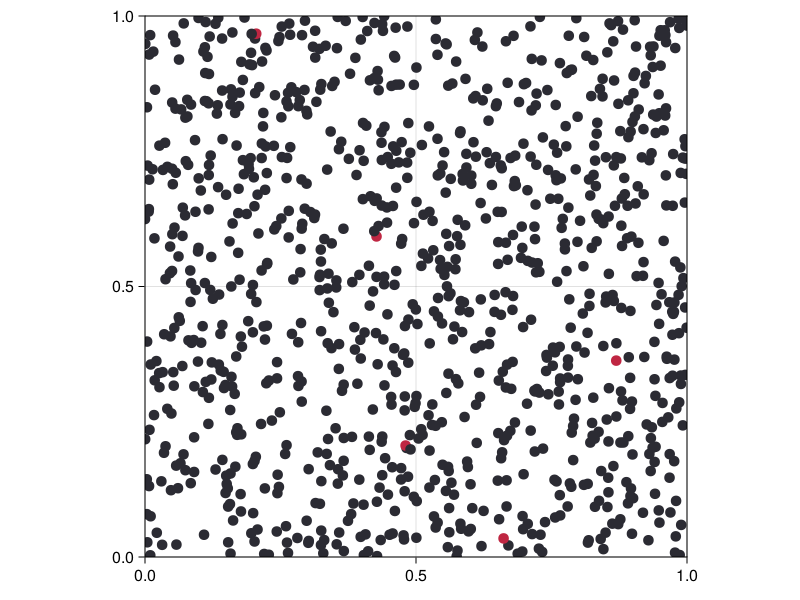
\includegraphics[width=\textwidth]{img/ball-covid.png}
    \captionof{figure}{Esempio del modello modellato su spazio continuo}
    \label{fig:ball_covid}
\end{minipage}

Sono state poi implementate svariate proprieta' come la proprieta' di essere individuati 
dopo un periodo di latenza come individui infetti e quindi essere confinati in quarantena, 
la quale era definita come una diminuzione nella probabilita' di infettare ed essere infettati 
perdendo la capacita' di muoversi.

Sono state implementate molti altri particolari approcci, la maggior parte Agent oriented.
Tuttavia questa tipologia di approccio richiedeva una quantita' di risorse computazionali 
e di tempo estremamente elevato in relazione al numero di agenti presenti nel modello. Questo approccio 
inoltre e' stato valutato come troppo granulare e inadatto allo scopo del progetto. 
Si e' deciso quindi di adottare un approccio meno granulare e piu' flessibile 
andando ad un livello di astrazione piu' alto.

\subsection{Modello ad Agente con spazio a grafo e modellazione singolo agente}
L'idea e' nata per cercare di avere un controllo piu' granulare sul modello e sulla sua 
evoluzione locale, non tanto degli agenti. Sono nati molteplici problemi, primo tra tutti quello del tempo impiegato
e successivamente quello del comportamento delle curve epidemiologiche che non rispettavano 
assolutamente il comportamento descritto dal modello deterministico SEIR, ma non in un modo 
ragionevole, bensi' in un modo completamente alieno e descritto brutalmente dalla
seguente formula 

\begin{minipage}{\linewidth}
    \centering
    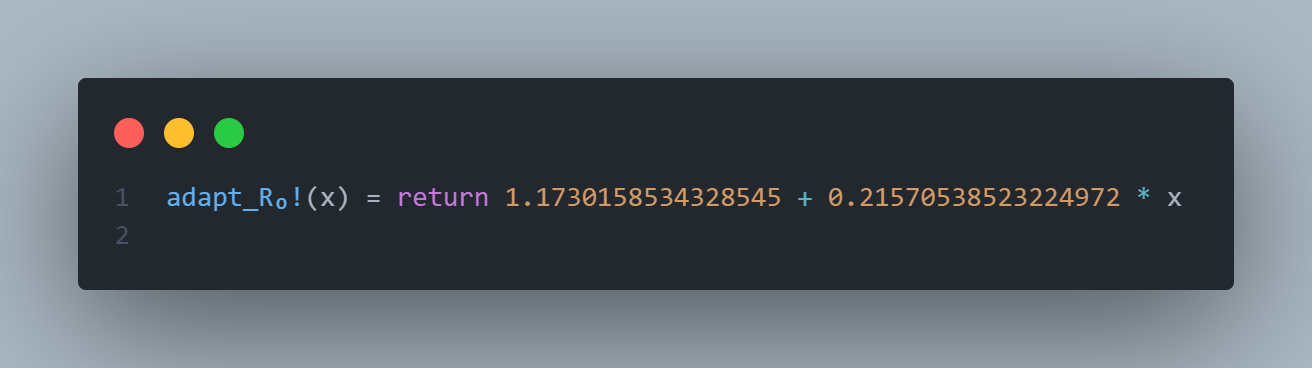
\includegraphics[width=\textwidth]{img/rapporto_strano.png}
    \captionof{figure}{Formula che si occupa di descrivere il rapporto tra il comportamento del modello scartato e del modello SEIR. In particolare questa formula descrive il rapporto tra gli $R_0$}
    \label{fig:strange_behaviour_R0}
\end{minipage}

In particolare la formula e' stata ricavata dopo aver fatto un confronto tra molteplici 
valori di $R_0$ e i risultati ottenuti sia dal modello SEIR che dal modello ABM. 
Successivamente e' stato calcolato \textbf{MSE} (Medium Square Error) per ogni coppia possibile
di risultati per cercare quelli tra loro piu' simili, andando ad ottenere quindi un insieme
di coppie. Queste poi sono state inserite in un metodo che calcolava una \textbf{polynomial fit}
tra tutte le coppie di valori per vedere quale poteva essere la formula che governava la differenza 
di risultati. Da tenere a mente che in un caso normale questa differenza non dovrebbe esiste, 
o quanto meno se esiste dovrebbe essere trascurabile.

Da qui si ottiene la formula in figura \ref{fig:strange_behaviour_R0}

\begin{figure}[!hb]
	\centering
	\begin{subfigure}[b]{0.45\textwidth}
		\centering
		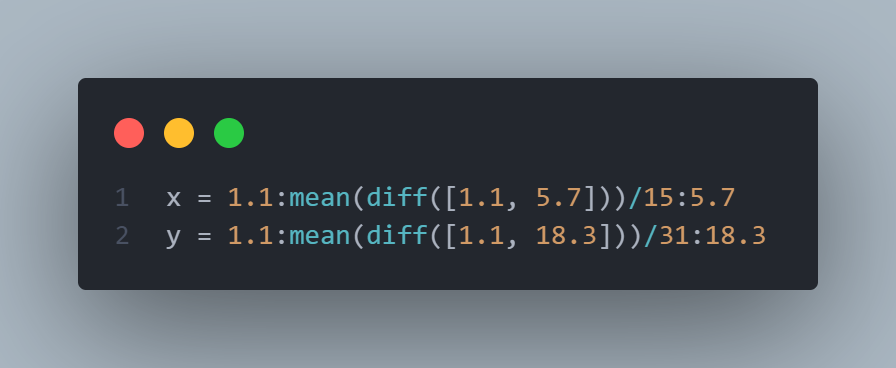
\includegraphics[width=\textwidth]{img/r0_range_test.png}
    	\caption{figure}{Range di valori di $R_0$ testati}
    	\label{fig:r0_range_test}
	\end{subfigure}
	\hfill
	\begin{subfigure}[b]{0.45\textwidth}
		\centering
		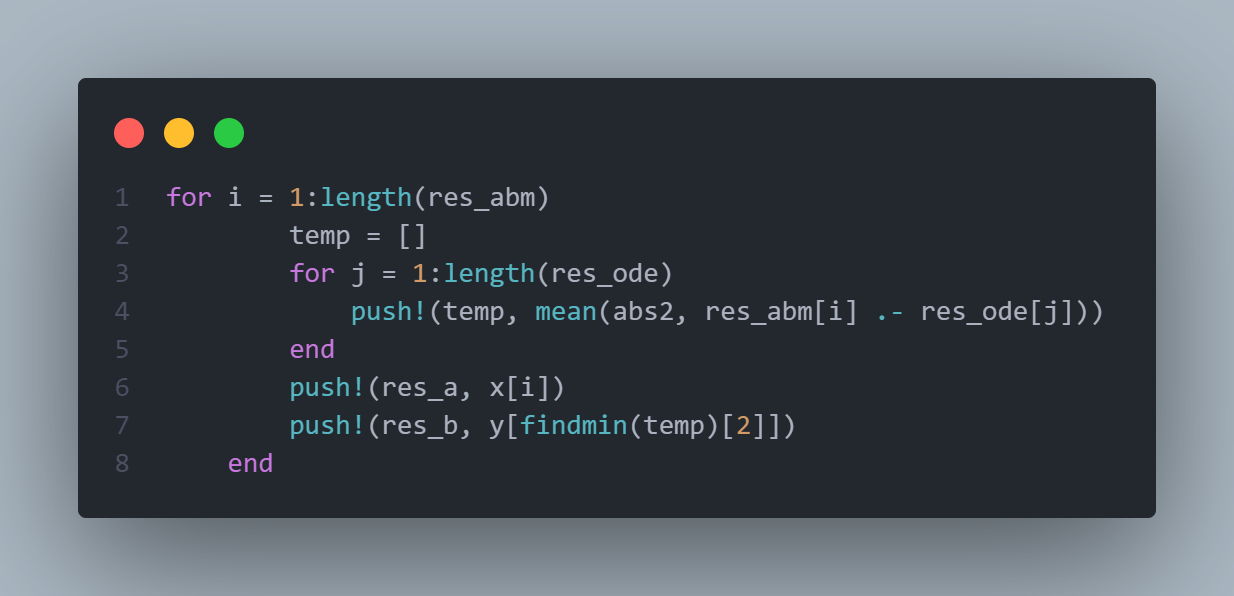
\includegraphics[width=\textwidth]{img/mse_r0.png}
		\caption{Calcolo MSE risultati SEIR - ABM}
		\label{fig:mse_r0}
	\end{subfigure}
\end{figure}

La motivazione per cui il modello ad agente si comporta in maniera cosi' inaspettata
rispetto a come dovrebbe non e' stato chiaro, e per questo ho deciso di abbandonare l'approccio.
Punto a favore e' stato anche il fatto che l'approccio con ABM era estremaente esoso in termini 
di risorse computazionali e tempistiche. Questo problema e' insito in ogni tipo di simulazione, 
tuttavia affiancato allo stravagante problema comparso e descritto sopra, e' stato 
decisivo per il cambio drastico di approccio. 